\chapter{Modelo de datos}
En este capítulo se estudiará la estructura de datos del sistema mediante un \textit{Modelo Entidad-Interrelación} (E-R).
Primero se identificarán y detallarán los tipos de entidad, luego los tipos de interrelación y finalmente se sintetizará todo el modelo en un diagrama E-R.

\section {Análisis de los tipos de entidad}\label{analisis-tipos-entidad}
Los tipos de entidad representan conceptos del mundo real. Las entidades son son instancias de dichos tipos. Una entidad se diferencia de cualquier otra incluso si las dos son del mismo tipo.
Los tipos de entidad pueden ser fuertes, si la existencia de sus entidades no depende de la existencia de otras en el dominio del problema, o débiles si para existir necesitan la existencia de una entidad fuerte. Así mismo, las entidades débiles pueden serlo por identificación o por existencia.

\subsection{Aplicaciones}
\subsubsection*{Descripción}
Este tipo de entidad representa las aplicaciones móviles de pushnews. Por cada aplicación registrada habrá una aplicación móvil en la tienda de aplicaciones de Google, de Apple o en ambas. Cada aplicación cuenta con un subdominio propio para acceder a pushnews, unas credenciales para el servicio de mensajería push, su propio logotipo y una APIKEY para verificar la autenticidad de las solicitudes al servicio web.

\subsubsection*{Restricciones}
No habrá aplicaciones con el mismo nombre tampoco con el mismo subdominio.

\subsubsection*{Características}
\begin{description}[nosep,style=multiline,labelindent=0.8cm,leftmargin=4.5cm,font=\normalfont]
    \item[Nombre] Aplicaciones
    \item[Id. principal] AplicacionID
    \item[Id. alternativo] Subdominio
    \item[Atrib. heredados] LogotipoID (Documentos)
\end{description}

\subsubsection*{Atributos de la entidad}
En la tabla \ref{cuadro:atributos-tipo-entidad-aplicaciones} se describen todos los atributos de la entidad. Así mismo, en la tabla \ref{cuadro:ejemplo-aplicacion} se muestra un ejemplo de los valores que tendría un registro de aplicación.

\begin{table}[h]
    \rowcolors{2}{gray!25}{white}
    \centering
    %\resizebox{\textwidth}{!}{%
    \begin{tabular}{|llcp{8.3cm}|}
        \hline
        \rowcolor[HTML]{9B9B9B}
        \multicolumn{1}{|l}{\cellcolor[HTML]{9B9B9B}{\color[HTML]{FFFFFF} Atributo}} & 
        \multicolumn{1}{c}{\cellcolor[HTML]{9B9B9B}{\color[HTML]{FFFFFF} Dominio}} &
        \multicolumn{1}{c}{\cellcolor[HTML]{9B9B9B}{\color[HTML]{FFFFFF} Obl.}} &
        \multicolumn{1}{c|}{\cellcolor[HTML]{9B9B9B}{\color[HTML]{FFFFFF} Descripción}} \\
        AplicacionID & $\mathbb N$ & \cmark & Identificador de aplicación \\
        Nombre & Alfanumérico & \cmark & Nombre de la aplicación \\
        Versión & Alfanumérico & \cmark & Versión de la aplicación \\
        Activo & Booleano & \cmark & Aplicación activa/inactiva \\
        SubDominio & Alfanumérico & \cmark & Subdominio de la aplicación \\
        CloudKey & Alfanumérico & \cmark & APIKEY del servicio de mensajería PUSH \\
        Usuario & Alfanumérico & \xmark & Usuario del servicio de mensajería PUSH \\
        Clave & Alfanumérico & \xmark & Contraseña del servicio de mensajería PUSH \\
        LogotipoID & $\mathbb N$ & \xmark & ID del documento con el logotipo \\
        ApiKey & Alfanumérico & \cmark & Clave de seguridad de la API.\\
        PlayStoreUrl & URL & \xmark & Url de la aplicación en la PlayStore \\
        AppStoreUrl & URL & \xmark & Url de la aplicación en la AppStore. \\
        \hline
    \end{tabular}%}
    \caption{Atributos del tipo de entidad Aplicaciones}
    \label{cuadro:atributos-tipo-entidad-aplicaciones}
\end{table} 

\begin{table}[h]
    \rowcolors{2}{gray!25}{white}
    \centering
    %\resizebox{\textwidth}{!}{%
    \begin{tabular}{|ll|}
        \hline
        \rowcolor[HTML]{9B9B9B} 
        \multicolumn{1}{|c}{\cellcolor[HTML]{9B9B9B}{\color[HTML]{FFFFFF} Atributo}} & \multicolumn{1}{c|}{\cellcolor[HTML]{9B9B9B}{\color[HTML]{FFFFFF} Valor}} \\ \hline
        AplicacionID & 1 \\
        Nombre & ``Escuela Politécnica Superior de Córdoba'' \\
        Versión & ``1.0.0.0'' \\
        Activo & Verdadero \\
        SubDominio & ``epsc'' \\
        CloudKey & <texto encriptado> \\
        Usuario & epspush \\
        Clave & <texto encriptado> \\
        LogotipoID & 8 \\
        ApiKey & `AIzaSyCqhjgrPTPSOFyLyos5gfN47TJ0HnNA\_LA' \\
        PlayStoreUrl & `https://play.google.com/\dots?id=com.pushnews.epsc' \\
        AppStoreUrl & `https://apps.apple.com/\dots/pushnews-epsc' \\
        \hline
    \end{tabular}%}
    \caption{Ejemplo de registro de tipo Aplicación}
    \label{cuadro:ejemplo-aplicacion}
\end{table}

\subsection{Usuarios}

\subsubsection*{Descripción}
Los usuarios del sistema tienen un email único y una clave para acceder. Además, se almacena su nombre y una marca para indicar si el email ha sido confirmado.

Los usuarios tienen un rol de editor o administrador. Un editor se vincula a una o varias aplicaciones en las que puede administrar los comunicados, categorías, etc. Los administradores gestionan las aplicaciones existentes, usuarios, parámetros del sistema\dots y también pueden actuar como editores dentro de cualquier aplicación.

\subsubsection*{Restricciones}
No habrá usuarios con el mismo email.

\subsubsection*{Características}
\begin{description}[nosep,style=multiline,labelindent=0.8cm,leftmargin=4.5cm,font=\normalfont]
    \item[Nombre] Usuarios
    \item[Id. principal] UsuarioID
    \item[Id. alternativo] Email
    \item[Atrib. heredados] RolID (Roles.RolID)
\end{description}

\subsubsection*{Atributos de la entidad}
En la tabla \ref{cuadro:atributos-tipo-entidad-usuarios} se describen todos los atributos de la entidad. Así mismo, en la tabla \ref{cuadro:ejemplo-usuario} se muestra un ejemplo de los valores que tendría un registro de usuario.

\begin{table}[h]
    \rowcolors{2}{gray!25}{white}
    \centering
    %\resizebox{\textwidth}{!}{%
    \begin{tabular}{|llcp{6.5cm}|}
        \hline
        \rowcolor[HTML]{9B9B9B}
        \multicolumn{1}{|l}{\cellcolor[HTML]{9B9B9B}{\color[HTML]{FFFFFF} Atributo}} & 
        \multicolumn{1}{c}{\cellcolor[HTML]{9B9B9B}{\color[HTML]{FFFFFF} Dominio}} &
        \multicolumn{1}{c}{\cellcolor[HTML]{9B9B9B}{\color[HTML]{FFFFFF} Obl.}} &
        \multicolumn{1}{c|}{\cellcolor[HTML]{9B9B9B}{\color[HTML]{FFFFFF} Descripción}} \\
        UsuarioID & $\mathbb N$ & \cmark & Identificador de usuario \\
        Email & Alfanumérico & \cmark & Email del usuario \\
        Nombre & Alfanumérico & \cmark & Nombre del usuario \\
        Apellidos & Alfanumérico & \cmark & Apellidos del usuario \\
        Clave & Alfanumérico & \cmark & Clave de acceso del usuario \\
        Activo & Booleano & \cmark & Aplicación activa/inactiva \\
        EmailConfirmado & Booleano & \cmark & El usuario ha confirmado el email \\
        Creado & Fecha & \cmark & Fecha de creación del registro \\
        Actualizado & Fecha & \xmark & Fecha de actualización del registro \\
        RolID & $\mathbb N$ & \cmark & ID del rol del usuario\\
        \hline
    \end{tabular}%}
    \caption{Atributos del tipo de entidad Usuarios}
    \label{cuadro:atributos-tipo-entidad-usuarios}
\end{table}


\begin{table}[h]
    \rowcolors{2}{gray!25}{white}
    \centering
    %\resizebox{\textwidth}{!}{%
    \begin{tabular}{|ll|}
        \hline
        \rowcolor[HTML]{9B9B9B} 
        \multicolumn{1}{|c}{\cellcolor[HTML]{9B9B9B}{\color[HTML]{FFFFFF} Atributo}} & \multicolumn{1}{c|}{\cellcolor[HTML]{9B9B9B}{\color[HTML]{FFFFFF} Valor}} \\ \hline
        UsuarioID & 1 \\
        Email & ``joselopez@mailsrv.com'' \\
        Nombre & ``José'' \\
        Apellidos & ``López Pérez'' \\
        Clave & <texto encriptado> \\
        Activo & Verdadero \\
        EmailConfirmado & Falso \\
        Creado & 2020-11-07 11:03:00 \\
        Actualizado & 2020-11-08 16:52:00 \\
        RolID & 1 \\
        \hline
    \end{tabular}%}
    \caption{Ejemplo de registro de tipo Usuario}
    \label{cuadro:ejemplo-usuario}
\end{table}

\subsection{Categorías}

\subsubsection*{Descripción}
Las categorías se definen para cada aplicación y agrupan los comunicados por temática. Tienen un nombre y un icono que las representa. Se ordenan según el criterio de los editores, para lo que cuentan con un campo orden. Pueden estar activas o inactivas. Si una categoría está inactiva, los comunicados de esta categoría no serán visibles ni se podrán crear nuevos comunicados en esta categoría.

\subsubsection*{Restricciones}
Ninguna

\subsubsection*{Características}
\begin{description}[nosep,style=multiline,labelindent=0.8cm,leftmargin=4.5cm,font=\normalfont]
    \item[Nombre] Usuarios
    \item[Id. principal] CategoriaID
    \item[Id. alternativo] Ninguno
    \item[Atrib. heredados] AplicacionID (Aplicaciones)
\end{description}

\subsubsection*{Atributos de la entidad}
En la tabla \ref{cuadro:atributos-tipo-entidad-categorias} se describen todos los atributos de la entidad. Así mismo, en la tabla \ref{cuadro:ejemplo-categoria} se muestra un ejemplo de los valores que tendría un registro de categoría.

\begin{table}[h]
    \rowcolors{2}{gray!25}{white}
    \centering
    %\resizebox{\textwidth}{!}{%
    \begin{tabular}{|llcp{8.3cm}|}
        \hline
        \rowcolor[HTML]{9B9B9B}
        \multicolumn{1}{|l}{\cellcolor[HTML]{9B9B9B}{\color[HTML]{FFFFFF} Atributo}} & 
        \multicolumn{1}{c}{\cellcolor[HTML]{9B9B9B}{\color[HTML]{FFFFFF} Dominio}} &
        \multicolumn{1}{c}{\cellcolor[HTML]{9B9B9B}{\color[HTML]{FFFFFF} Obl.}} &
        \multicolumn{1}{c|}{\cellcolor[HTML]{9B9B9B}{\color[HTML]{FFFFFF} Descripción}} \\
        CategoriaID & $\mathbb N$ & \cmark & Identificador de la categoría \\
        AplicaciónID & $\mathbb N$ & \cmark & Identificador de la aplicación de la categoría \\
        Nombre & Alfanumérico & \cmark & Nombre de la categoría \\
        Icono & Alfanumérico & \cmark & Icono (fontawesome) de la categoría \\
        Orden & $\mathbb N$ & \cmark & Orden de la categoría \\
        Activo & Booleano & \cmark & Comunicado activo/inactivo \\
        \hline
    \end{tabular}%}
    \caption{Atributos del tipo de entidad Categorías}
    \label{cuadro:atributos-tipo-entidad-categorias}
\end{table}

\begin{table}[h]
    \rowcolors{2}{gray!25}{white}
    \centering
    %\resizebox{\textwidth}{!}{%
    \begin{tabular}{|ll|}
        \hline
        \rowcolor[HTML]{9B9B9B} 
        \multicolumn{1}{|c}{\cellcolor[HTML]{9B9B9B}{\color[HTML]{FFFFFF} Atributo}} & \multicolumn{1}{c|}{\cellcolor[HTML]{9B9B9B}{\color[HTML]{FFFFFF} Valor}} \\ \hline
        CategoriaID & 17 \\
        AplicacionID & 3 \\
        Nombre & ``Secretaría'' \\
        Icono & ``fa-leanpub'' \\
        Orden & 3 \\
        Activo & Verdadero \\
        \hline
    \end{tabular}
    \caption{Ejemplo de registro de tipo Categorías}
    \label{cuadro:ejemplo-categoria}
\end{table}

\subsection{Características de aplicaciones}

\subsubsection*{Descripción}
Las características son funcionalidades que se pueden habilitar o deshabilitar para cada aplicación. Ejemplos de características serían la posibilidad de incrustar un vídeo de Youtube en los comunicados o el acceso al módulo de directorio comercial.

\subsubsection*{Restricciones}
No habrá dos características con el mismo nombre.

\subsubsection*{Características}
\begin{description}[nosep,style=multiline,labelindent=0.8cm,leftmargin=4.5cm,font=\normalfont]
    \item[Nombre] AplicacionesCaracteristicas
    \item[Id. principal] AplicacionCaracteristicaID
    \item[Id. alternativo] Ninguno
    \item[Atrib. heredados] Ninguno
\end{description}

\subsubsection*{Atributos de la entidad}
En la tabla \ref{cuadro:atributos-tipo-entidad-caracteristicas} se describen todos los atributos de la entidad. Así mismo, en la tabla \ref{cuadro:ejemplo-caracteristica} se muestra un ejemplo de los valores que tendría un registro de característica.

\begin{table}[h]
    \rowcolors{2}{gray!25}{white}
    \centering
    %\resizebox{\textwidth}{!}{%
    \begin{tabular}{|llcp{5.9cm}|}
        \hline
        \rowcolor[HTML]{9B9B9B}
        \multicolumn{1}{|l}{\cellcolor[HTML]{9B9B9B}{\color[HTML]{FFFFFF} Atributo}} & 
        \multicolumn{1}{c}{\cellcolor[HTML]{9B9B9B}{\color[HTML]{FFFFFF} Dominio}} &
        \multicolumn{1}{c}{\cellcolor[HTML]{9B9B9B}{\color[HTML]{FFFFFF} Obl.}} &
        \multicolumn{1}{c|}{\cellcolor[HTML]{9B9B9B}{\color[HTML]{FFFFFF} Descripción}} \\
        AplicacionCaracteristicaID & $\mathbb N$ & \cmark & Identificador de la característica \\
        Nombre & Alfanumérico & \cmark & Nombre de la característica \\
        Activo & Booleano & \cmark & Característica activa/inactiva \\
        \hline
    \end{tabular}%}
    \caption{Atributos del tipo de entidad Características}
    \label{cuadro:atributos-tipo-entidad-caracteristicas}
\end{table}

\begin{table}[h]
    \rowcolors{2}{gray!25}{white}
    \centering
    %\resizebox{\textwidth}{!}{%
    \begin{tabular}{|ll|}
        \hline
        \rowcolor[HTML]{9B9B9B} 
        \multicolumn{1}{|c}{\cellcolor[HTML]{9B9B9B}{\color[HTML]{FFFFFF} Atributo}} & \multicolumn{1}{c|}{\cellcolor[HTML]{9B9B9B}{\color[HTML]{FFFFFF} Valor}} \\ \hline
        AplicacionCaracteristicaID & 4 \\
        Nombre & ``DirectorioComercial'' \\
        Activo & Verdadero \\
        \hline
    \end{tabular}
    \caption{Ejemplo de registro de tipo Características}
    \label{cuadro:ejemplo-caracteristica}
\end{table}

\subsection{Terminales}

\subsubsection*{Descripción}
Los terminales son los dispositivos o navegadores que utilizan los lectores para acceder a los comunicados. Un terminal se registra en el sistema la primera vez que solicita la lectura de un comunicado, relacionado con la aplicación que está utilizando. Se guarda la fecha y la IP de la última conexión del dispositivo.

\subsubsection*{Restricciones}
Ninguna.

\subsubsection*{Características}
\begin{description}[nosep,style=multiline,labelindent=0.8cm,leftmargin=4.5cm,font=\normalfont]
    \item[Nombre] Terminales
    \item[Id. principal] TerminalID
    \item[Id. alternativo] Ninguno
    \item[Atrib. heredados] AplicacionID (Aplicaciones)
\end{description}

\subsubsection*{Atributos de la entidad}
En la tabla \ref{cuadro:atributos-tipo-entidad-terminales} se describen todos los atributos de la entidad. Así mismo, en la tabla \ref{cuadro:ejemplo-terminal} se muestra un ejemplo de los valores que tendría un registro de terminal.

\begin{table}[h]
    \rowcolors{2}{gray!25}{white}
    \centering
    %\resizebox{\textwidth}{!}{%
    \begin{tabular}{|llcp{5.5cm}|}
        \hline
        \rowcolor[HTML]{9B9B9B}
        \multicolumn{1}{|l}{\cellcolor[HTML]{9B9B9B}{\color[HTML]{FFFFFF} Atributo}} & 
        \multicolumn{1}{c}{\cellcolor[HTML]{9B9B9B}{\color[HTML]{FFFFFF} Dominio}} &
        \multicolumn{1}{c}{\cellcolor[HTML]{9B9B9B}{\color[HTML]{FFFFFF} Obl.}} &
        \multicolumn{1}{c|}{\cellcolor[HTML]{9B9B9B}{\color[HTML]{FFFFFF} Descripción}} \\
        TerminalID & $\mathbb N$ & \cmark & Identificador del terminal \\
        AplicacionID & $\mathbb N$ & \cmark & Identificador de la aplicación \\
        Nombre & Alfanumérico & \cmark & Nombre del terminal \\
        UltimaConexionFecha & Fecha & \cmark & Fecha de la última conexión \\
        UltimaConexionIP & Alfanumérico & \xmark & IP de la última conexión \\
        \hline
    \end{tabular}%}
    \caption{Atributos del tipo de entidad Terminales}
    \label{cuadro:atributos-tipo-entidad-terminales}
\end{table}

\begin{table}[h]
    \rowcolors{2}{gray!25}{white}
    \centering
    %\resizebox{\textwidth}{!}{%
    \begin{tabular}{|ll|}
        \hline
        \rowcolor[HTML]{9B9B9B} 
        \multicolumn{1}{|c}{\cellcolor[HTML]{9B9B9B}{\color[HTML]{FFFFFF} Atributo}} & \multicolumn{1}{c|}{\cellcolor[HTML]{9B9B9B}{\color[HTML]{FFFFFF} Valor}} \\ \hline
        TerminalID & 4 \\
        AplicacionID & 17 \\
        Nombre & <UID-del-dispositivo> \\
        UltimaConexionFecha & 2020-11-08 11:32:14 \\
        UltimaConexionIP & ``87.30.18.207'' \\
        \hline
    \end{tabular}
    \caption{Ejemplo de registro de tipo Terminal}
    \label{cuadro:ejemplo-terminal}
\end{table}

\subsection{Documentos}

\subsubsection*{Descripción}
Documento es cualquier archivo que se adjunte a otras entidades como Comunicados, Aplicaciones (logotipo), etc. Este tipo de entidad es el catálogo de los archivos en disco que están asociados a contenidos del sistema. Los documentos se registran asociados a la aplicación a la que pertenecen y mantienen información sobre la ruta en disco, el nombre del recurso, el tipo MIME, el tamaño y la fecha de creación. Los documentos pueden ser de dos tipos: Adjunto e Imagen. La lista de tipos está pensada para añadir fácilmente otros tipos en caso de que surja la necesidad.

\subsubsection*{Restricciones}
Ninguna

\subsubsection*{Características}
\begin{description}[nosep,style=multiline,labelindent=0.8cm,leftmargin=4.5cm,font=\normalfont]
    \item[Nombre] Documentos
    \item[Id. principal] DocumentoID
    \item[Id. alternativo] Ninguno
    \item[Atrib. heredados] AplicacionID (Aplicaciones)
\end{description}

\subsubsection*{Atributos de la entidad}
En la tabla \ref{cuadro:atributos-tipo-entidad-documentos} se describen todos los atributos de la entidad. Así mismo, en la tabla \ref{cuadro:ejemplo-documento} se muestra un ejemplo de los valores que tendría un registro de documento.

\begin{table}[h]
    \rowcolors{2}{gray!25}{white}
    \centering
    %\resizebox{\textwidth}{!}{%
    \begin{tabular}{|llcp{6.2cm}|}
        \hline
        \rowcolor[HTML]{9B9B9B}
        \multicolumn{1}{|l}{\cellcolor[HTML]{9B9B9B}{\color[HTML]{FFFFFF} Atributo}} & 
        \multicolumn{1}{c}{\cellcolor[HTML]{9B9B9B}{\color[HTML]{FFFFFF} Dominio}} &
        \multicolumn{1}{c}{\cellcolor[HTML]{9B9B9B}{\color[HTML]{FFFFFF} Obl.}} &
        \multicolumn{1}{c|}{\cellcolor[HTML]{9B9B9B}{\color[HTML]{FFFFFF} Descripción}} \\
        DocumentoID & $\mathbb N$ & \cmark & Identificador del documento \\
        AplicacionID & $\mathbb N$ & \cmark & Identificador de la aplicación \\
        Tipo & $\mathbb N$ & \cmark & Tipo de documento \\
        Nombre & Alfanumérico & \cmark & Nombre del archivo al descargar \\
        Ruta & Ruta de disco & \cmark & Ruta del archivo \\
        Mime & Tipos MIME & \cmark & Tipo MIME del archivo \\
        Tamaño & $\mathbb R > 0$ & \cmark & Tamaño del fichero en MB \\
        Fecha & Fecha & \cmark & Fecha de creación \\
        \hline
    \end{tabular}%}
    \caption{Atributos del tipo de entidad Documentos}
    \label{cuadro:atributos-tipo-entidad-documentos}
\end{table}

\begin{table}[h]
    \rowcolors{2}{gray!25}{white}
    \centering
    %\resizebox{\textwidth}{!}{%
    \begin{tabular}{|ll|}
        \hline
        \rowcolor[HTML]{9B9B9B} 
        \multicolumn{1}{|c}{\cellcolor[HTML]{9B9B9B}{\color[HTML]{FFFFFF} Atributo}} & \multicolumn{1}{c|}{\cellcolor[HTML]{9B9B9B}{\color[HTML]{FFFFFF} Valor}} \\ \hline
        DocumentoID & 84 \\
        AplicacionID & 6 \\
        Tipo & 1 \\
        Nombre & ``CartelJornadas.png'' \\
        Ruta & ``6/CartelJornadas\_H2NF67.png'' \\
        Mime & image/png \\
        Tamaño & 3,6 \\
        Fecha & 2020-11-14 13:22:41 \\
        \hline
    \end{tabular}
    \caption{Ejemplo de registro de tipo Documento}
    \label{cuadro:ejemplo-documento}
\end{table}

\subsection{Roles}

\subsubsection*{Descripción}
Esta entidad representa los tipos de privilegios de acceso que pueden tener los usuarios.

\subsubsection*{Restricciones}
Ninguna

\subsubsection*{Características}
\begin{description}[nosep,style=multiline,labelindent=0.8cm,leftmargin=4.5cm,font=\normalfont]
    \item[Nombre] Roles
    \item[Id. principal] RolID
    \item[Id. alternativo] Ninguno
    \item[Atrib. heredados] Ninguno
\end{description}

\subsubsection*{Atributos de la entidad}
En la tabla \ref{cuadro:atributos-tipo-entidad-roles} se describen todos los atributos de la entidad. Así mismo, en la tabla \ref{cuadro:ejemplo-rol} se muestra un ejemplo de los valores que tendría un registro de documento.

\begin{table}[h]
    \rowcolors{2}{gray!25}{white}
    \centering
    %\resizebox{\textwidth}{!}{%
    \begin{tabular}{|llcp{5.9cm}|}
        \hline
        \rowcolor[HTML]{9B9B9B}
        \multicolumn{1}{|l}{\cellcolor[HTML]{9B9B9B}{\color[HTML]{FFFFFF} Atributo}} & 
        \multicolumn{1}{c}{\cellcolor[HTML]{9B9B9B}{\color[HTML]{FFFFFF} Dominio}} &
        \multicolumn{1}{c}{\cellcolor[HTML]{9B9B9B}{\color[HTML]{FFFFFF} Obl.}} &
        \multicolumn{1}{c|}{\cellcolor[HTML]{9B9B9B}{\color[HTML]{FFFFFF} Descripción}} \\
        RolID & $\mathbb N$ & \cmark & Identificador del rol \\
        Nombre & Alfanumérico & \cmark & Nombre del rol \\
        \hline
    \end{tabular}%}
    \caption{Atributos del tipo de entidad Roles}
    \label{cuadro:atributos-tipo-entidad-roles}
\end{table}

\begin{table}[h]
    \rowcolors{2}{gray!25}{white}
    \centering
    %\resizebox{\textwidth}{!}{%
    \begin{tabular}{|ll|}
        \hline
        \rowcolor[HTML]{9B9B9B} 
        \multicolumn{1}{|c}{\cellcolor[HTML]{9B9B9B}{\color[HTML]{FFFFFF} Atributo}} & \multicolumn{1}{c|}{\cellcolor[HTML]{9B9B9B}{\color[HTML]{FFFFFF} Valor}} \\ \hline
        RolID & 1 \\
        Nombre & ``Administrador'' \\
        \hline
    \end{tabular}
    \caption{Ejemplo de registro de tipo Rol}
    \label{cuadro:ejemplo-rol}
\end{table}

\subsection{Localizaciones}

\subsubsection*{Descripción}
Las localizaciones representan lugares de interés para los usuarios de la aplicación. Por ejemplo, para la aplicación de un Ayuntamiento, ejemplos de localizaciones serían la oficina de información turística, la dirección del propio Ayuntamiento, la comisaría de policía, etc. Las localizaciones contienen datos como las coordenadas, la dirección y la descripción de un lugar.

\subsubsection*{Restricciones}
Ninguna

\subsubsection*{Características}
\begin{description}[nosep,style=multiline,labelindent=0.8cm,leftmargin=4.5cm,font=\normalfont]
    \item[Nombre] Localizaciones
    \item[Id. principal] LocalizacionID
    \item[Id. alternativo] Ninguno
    \item[Atrib. heredados] AplicacionID (Aplicaciones)
\end{description}

\subsubsection*{Atributos de la entidad}
En la tabla \ref{cuadro:atributos-tipo-entidad-localizaciones} se describen todos los atributos de la entidad. Así mismo, en la tabla \ref{cuadro:ejemplo-localizacion} se muestra un ejemplo de los valores que tendría un registro de localización.

\begin{table}[h]
    \rowcolors{2}{gray!25}{white}
    \centering
    %\resizebox{\textwidth}{!}{%
    \begin{tabular}{|llcp{7.2cm}|}
        \hline
        \rowcolor[HTML]{9B9B9B}
        \multicolumn{1}{|l}{\cellcolor[HTML]{9B9B9B}{\color[HTML]{FFFFFF} Atributo}} & 
        \multicolumn{1}{c}{\cellcolor[HTML]{9B9B9B}{\color[HTML]{FFFFFF} Dominio}} &
        \multicolumn{1}{c}{\cellcolor[HTML]{9B9B9B}{\color[HTML]{FFFFFF} Obl.}} &
        \multicolumn{1}{c|}{\cellcolor[HTML]{9B9B9B}{\color[HTML]{FFFFFF} Descripción}} \\
        LocalizacionID & $\mathbb N$ & \cmark & Identificador de la localización \\
        AplicacionID & $\mathbb N$ & \cmark & Identificador de la aplicación asociada \\
        Fecha & Fecha & \cmark & Fecha de creación \\
        Longitud & $\mathbb R\in[-180, 180]$ & \cmark & Coordenadas: Longitud \\
        Latitud & $\mathbb R\in[-90, 90]$ & \cmark & Coordenadas: Latitud \\
        Descripción & Alfanumérico & \cmark & Descripción de la localización \\
        Activo & Booleano & \cmark & Localización activa/inactiva \\
        \hline
    \end{tabular}%}
    \caption{Atributos del tipo de entidad Localizaciones}
    \label{cuadro:atributos-tipo-entidad-localizaciones}
\end{table}

\begin{table}[h]
    \rowcolors{2}{gray!25}{white}
    \centering
    %\resizebox{\textwidth}{!}{%
    \begin{tabular}{|ll|}
        \hline
        \rowcolor[HTML]{9B9B9B} 
        \multicolumn{1}{|c}{\cellcolor[HTML]{9B9B9B}{\color[HTML]{FFFFFF} Atributo}} & \multicolumn{1}{c|}{\cellcolor[HTML]{9B9B9B}{\color[HTML]{FFFFFF} Valor}} \\ \hline
        LocalizacionID & 35 \\
        AplicacionID & 14 \\
        Fecha & 2020-12-06 18:42:14 \\
        Longitud & -5.074807 \\
        Latitud & 37.536277 \\
        Descripción & ``Centro de salud''\\
        Activo & Verdadero \\
        \hline
    \end{tabular}%}
    \caption{Ejemplo de registro de tipo Localización}
    \label{cuadro:ejemplo-localizacion}
\end{table}

\subsection{Teléfonos}

\subsubsection*{Descripción}
Los teléfonos representan teléfonos de interés para los usuarios de la aplicación. Por ejemplo, para la aplicación de un Ayuntamiento, ejemplos de localizaciones serían el teléfono de información turística, el de atención al público del Ayuntamiento, el del museo municipal\dots Los datos que contiene un registro de esta entidad son el número telefónico y la descripción.

\subsubsection*{Restricciones}
Ninguna

\subsubsection*{Características}
\begin{description}[nosep,style=multiline,labelindent=0.8cm,leftmargin=4.5cm,font=\normalfont]
    \item[Nombre] Telefonos
    \item[Id. principal] TelefonoID
    \item[Id. alternativo] Ninguno
    \item[Atrib. heredados] AplicacionID (Aplicaciones)
\end{description}

\subsubsection*{Atributos de la entidad}
En la tabla \ref{cuadro:atributos-tipo-entidad-telefonos} se describen todos los atributos de la entidad. Así mismo, en la tabla \ref{cuadro:ejemplo-telefono} se muestra un ejemplo de los valores que tendría un registro de teléfono.

\begin{table}[h]
    \rowcolors{2}{gray!25}{white}
    \centering
    %\resizebox{\textwidth}{!}{%
    \begin{tabular}{|llcp{7.2cm}|}
        \hline
        \rowcolor[HTML]{9B9B9B}
        \multicolumn{1}{|l}{\cellcolor[HTML]{9B9B9B}{\color[HTML]{FFFFFF} Atributo}} & 
        \multicolumn{1}{c}{\cellcolor[HTML]{9B9B9B}{\color[HTML]{FFFFFF} Dominio}} &
        \multicolumn{1}{c}{\cellcolor[HTML]{9B9B9B}{\color[HTML]{FFFFFF} Obl.}} &
        \multicolumn{1}{c|}{\cellcolor[HTML]{9B9B9B}{\color[HTML]{FFFFFF} Descripción}} \\
        TelefonoID & $\mathbb N$ & \cmark & Identificador del teléfono \\
        AplicacionID & $\mathbb N$ & \cmark & Identificador de la aplicación asociada \\
        Fecha & Fecha & \cmark & Fecha de creación \\
        Numero & Alfanumérico & \cmark & Número de teléfono \\
        Descripción & Alfanumérico & \cmark & Descripción del teléfono \\
        Activo & Booleano & \cmark & Teléfono activo/inactivo \\
        \hline
    \end{tabular}%}
    \caption{Atributos del tipo de entidad Teléfonos}
    \label{cuadro:atributos-tipo-entidad-telefonos}
\end{table}

\begin{table}[h]
    \rowcolors{2}{gray!25}{white}
    \centering
    %\resizebox{\textwidth}{!}
    \caption{Ejemplo de registro de tipo Teléfono}
    \label{cuadro:ejemplo-telefono}
\end{table}

\subsection{Parámetros}

\subsubsection*{Descripción}
Esta entidad almacena parámetros de configuración del sistema. Un parámetro puede ser global o puede declararse para una determinada aplicación si se establece un valor en el campo AplicacionID.

\subsubsection*{Restricciones}
Ninguna

\subsubsection*{Características}
\begin{description}[nosep,style=multiline,labelindent=0.8cm,leftmargin=4.5cm,font=\normalfont]
    \item[Nombre] Parametros
    \item[Id. principal] ParametroID
    \item[Id. alternativo] Nombre, AplicacionID
    \item[Atrib. heredados] AplicacionID (Aplicaciones)
\end{description}

\subsubsection*{Atributos de la entidad}
En la tabla \ref{cuadro:atributos-tipo-entidad-parametros} se describen todos los atributos de la entidad. Así mismo, en la tabla \ref{cuadro:ejemplo-parametro} se muestra un ejemplo de los valores que tendría un registro de parámetro.

\begin{table}[h!]
    \rowcolors{2}{gray!25}{white}
    \centering
    %\resizebox{\textwidth}{!}{%
    \begin{tabular}{|llcp{7.2cm}|}
        \hline
        \rowcolor[HTML]{9B9B9B}
        \multicolumn{1}{|l}{\cellcolor[HTML]{9B9B9B}{\color[HTML]{FFFFFF} Atributo}} & 
        \multicolumn{1}{c}{\cellcolor[HTML]{9B9B9B}{\color[HTML]{FFFFFF} Dominio}} &
        \multicolumn{1}{c}{\cellcolor[HTML]{9B9B9B}{\color[HTML]{FFFFFF} Obl.}} &
        \multicolumn{1}{c|}{\cellcolor[HTML]{9B9B9B}{\color[HTML]{FFFFFF} Descripción}} \\
        ParámetroID & $\mathbb N$ & \cmark & Identificador del parámetro \\
        AplicacionID & $\mathbb N$ & \xmark & Identificador de la aplicación asociada \\
        Nombre & Alfanumérico & \cmark & Nombre del parámetro \\
        Valor & Alfanumérico & \xmark & Valor del parámetro \\
        Descripcion & Alfanumérico & \xmark & Descripción del parámetro \\
        \hline
    \end{tabular}%}
    \caption{Atributos del tipo de entidad Parámetros}
    \label{cuadro:atributos-tipo-entidad-parametros}
\end{table}

\begin{table}[h]
    \rowcolors{2}{gray!25}{white}
    \centering
    %\resizebox{\textwidth}{!}
    \caption{Ejemplo de registro de tipo Parámetro}
    \label{cuadro:ejemplo-parametro}
\end{table} 

\subsection{Empresas}

\subsubsection*{Descripción}
Esta entidad almacena datos de empresas que se anuncian en la aplicación. Los datos almacenados son, por ejemplo, nombre, dirección, teléfono, coordenadas, email, banner, logotipo\dots

\subsubsection*{Restricciones}
Ninguna

\subsubsection*{Características}
\begin{description}[nosep,style=multiline,labelindent=0.8cm,leftmargin=4.5cm,font=\normalfont]
    \item[Nombre] Empresas
    \item[Id. principal] EmpresaID
    \item[Id. alternativo] Ninguno
    \item[Atrib. heredados]
        AplicacionID (Aplicaciones)
    
        LogotipoDocumentoID (Documentos)
        
        BannerDocumentoID (Documentos)
\end{description}

\subsubsection*{Atributos de la entidad}
En la tabla \ref{cuadro:atributos-tipo-entidad-empresas} se describen todos los atributos de la entidad. Así mismo, en la tabla \ref{cuadro:ejemplo-empresa} se muestra un ejemplo de los valores que tendría un registro de empresa.

\begin{table}[h!]
    \rowcolors{2}{gray!25}{white}
    \centering
    %\resizebox{\textwidth}{!}{%
    \begin{tabular}{|llcp{6.5cm}|}
        \hline
        \rowcolor[HTML]{9B9B9B}
        \multicolumn{1}{|l}{\cellcolor[HTML]{9B9B9B}{\color[HTML]{FFFFFF} Atributo}} & 
        \multicolumn{1}{c}{\cellcolor[HTML]{9B9B9B}{\color[HTML]{FFFFFF} Dominio}} &
        \multicolumn{1}{c}{\cellcolor[HTML]{9B9B9B}{\color[HTML]{FFFFFF} Obl.}} &
        \multicolumn{1}{c|}{\cellcolor[HTML]{9B9B9B}{\color[HTML]{FFFFFF} Descripción}} \\
        EmpresaID & $\mathbb N$ & \cmark & Identificador de la empresa \\
        AplicacionID & $\mathbb N$ & \xmark & Identificador de la aplicación asociada \\
        Nombre & Alfanumérico & \cmark & Nombre del parámetro \\
        Dirección & Alfanumérico & \xmark & Dirección postal \\
        Localidad & Alfanumérico & \xmark & Localidad de la dirección \\
        Provincia & Alfanumérico & \xmark & Provincia de la dirección \\
        Latitud & Alfanumérico & \xmark & Latitud de la dirección \\
        Longitud & Alfanumérico & \xmark & Longitud de la dirección \\
        Telefono & Alfanumérico & \xmark & Número de teléfono \\
        Email & Alfanumérico & \xmark & Email de contacto \\
        Web & Alfanumérico & \xmark & URL de la web \\
        Facebook & Alfanumérico & \xmark & URL de la página de Facebook \\
        Twitter & Alfanumérico & \xmark & URL de la página de Twitter \\
        LogotipoDocumentoID & $\mathbb N$ & \xmark & ID del documento con el logotipo \\
        BannerDocumentoID & $\mathbb N$ & \xmark & ID del documento con el banner \\
        Descripcion & $\mathbb N$ & \xmark & Descripción de la empresa \\
        Tags & Alfanumérico & \xmark & Tags para clasificación \\
        Activo & Booleano & \cmark & Empresa activa/inactiva \\
        \hline
    \end{tabular}%}
    \caption{Atributos del tipo de entidad Empresas}
    \label{cuadro:atributos-tipo-entidad-empresas}
\end{table}

\begin{table}[h]
    \rowcolors{2}{gray!25}{white}
    \centering
    %\resizebox{\textwidth}{!}{%
    \begin{tabular}{|ll|}
        \hline
        \rowcolor[HTML]{9B9B9B} 
        \multicolumn{1}{|c}{\cellcolor[HTML]{9B9B9B}{\color[HTML]{FFFFFF} Atributo}} &
        \multicolumn{1}{c|}{\cellcolor[HTML]{9B9B9B}{\color[HTML]{FFFFFF} Valor}} \\
        \hline
        EmpresaID & 91 \\
        AplicacionID & 14 \\
        Nombre & ``Librería Gutemberg'' \\
        Dirección & ``Calle Alborada 123'' \\
        Localidad & ``Santaella'' \\
        Provincia & ``Córdoba'' \\
        Latitud & 37.913484 \\
        Longitud & -4.721551 \\
        Telefono & ``957456789'' \\
        Email & ``info@gutemberglibreria.es'' \\
        Web & ``http://www.gutemberglibreria.es'' \\
        Facebook & ``http://facebook.com/gutemberglibreria'' \\
        Twitter & ``http://twitter.com/gutemberglibreria'' \\
        LogotipoDocumentoID & 467 \\
        BannerDocumentoID & 236 \\
        Descripcion & ``Librería Gutemberg, prensa y papelería.'' \\
        Tags & ``libro,literatura,cultura,comercio'' \\
        Activo & Verdadero \\
        \hline
    \end{tabular}%}
    \caption{Ejemplo de registro de tipo Empresa}
    \label{cuadro:ejemplo-empresa}
\end{table}

\subsection{Comunicados}

\subsubsection*{Descripción}
Un comunicado es una publicación realizada por un editor en una aplicación. El comunicado contiene datos sobre su contenido como título, cuerpo, categoría y recursos adjuntos como enlaces, documentos o imágenes, fecha de publicación, etc. Además, tiene otros datos como su estado (publicada, borrada, activa...), estado de notificaciones push (notificada o no, recordatorio...). Los comunicados podrán ser inmediatas si se publican inmediatamente o programadas, cuando se programan para ser publicadas en una fecha y hora concretas.

\subsubsection*{Restricciones}
No habrá usuarios con el mismo email.

\subsubsection*{Características}
\begin{description}[nosep,style=multiline,labelindent=0.8cm,leftmargin=4.5cm,font=\normalfont]
    \item[Nombre] Comunicados
    \item[Id. principal] ComunicadoID
    \item[Id. alternativo] Ninguno
    \item[Atrib. heredados] 
        UsuarioID (Usuarios)

        CategoriaID (Categorias)

        ImagenDocumentoID (Documentos)

        AdjuntoDocumentoID (Documentos)
\end{description}

\subsubsection*{Atributos de la entidad}
En la tabla \ref{cuadro:atributos-tipo-entidad-comunicados} se describen todos los atributos de la entidad. Así mismo, en la tabla \ref{cuadro:ejemplo-comunicados} se muestra un ejemplo de los valores que tendría un registro de característica.

\begin{table}[h!]
    \rowcolors{2}{gray!25}{white}
    \centering
    %\resizebox{\textwidth}{!}{%
    \begin{tabular}{|llcp{6.7cm}|}
        \hline
        \rowcolor[HTML]{9B9B9B}
        \multicolumn{1}{|l}{\cellcolor[HTML]{9B9B9B}{\color[HTML]{FFFFFF} Atributo}} & 
        \multicolumn{1}{c}{\cellcolor[HTML]{9B9B9B}{\color[HTML]{FFFFFF} Dominio}} &
        \multicolumn{1}{c}{\cellcolor[HTML]{9B9B9B}{\color[HTML]{FFFFFF} Obl.}} &
        \multicolumn{1}{c|}{\cellcolor[HTML]{9B9B9B}{\color[HTML]{FFFFFF} Descripción}} \\
        ComunicadoID & $\mathbb N$ & \cmark & Identificador del comunicado \\
        UsuarioID & $\mathbb N$ & \cmark & Identificador del usuario editor \\
        CategoriaID & $\mathbb N$ & \cmark & Identificador de la categoría del comunicado \\
        FechaCreacion & Fecha & \cmark & Fecha de creación \\
        FechaPublicacion & Fecha & \cmark & Fecha de publicación \\
        Activo & Booleano & \cmark & Comunicado activo/inactivo \\
        Borrado & Booleano & \cmark & Marca de borrado del comunicado \\
        FechaBorrado & Fecha & \xmark & Fecha de borrado del comunicado \\
        TimeStamp & $\mathbb N$ & \xmark & Marca de tiempo de la publicación \\
        PushEnviada & Booleano & \cmark & Notificación push enviada/no enviada \\
        PushFecha & Fecha & \xmark & Fecha de notificación push \\
        Titulo & Alfanumérico & \cmark & Título del comunicado \\
        Descripcion & Booleano & \cmark & Cuerpo del comunicado \\
        UltimaEdicionIP & Alfanumérico & \xmark & IP desde la que se realizó la última edición \\
        Autor & Alfanumérico & \cmark & Nombre del autor \\
        Destacado & Booleano & \cmark & Publicación destacada/no destacada \\
        RecordatorioTitulo & Alfanumérico & \xmark & Texto del recordatorio \\
        RecordatorioFecha & Fecha & \xmark & Fecha del mensaje recordatorio \\
        PushRecordatorio & Booleano & \xmark & Mensaje push del recordatorio enviado/no enviado \\
        Instantanea & Booleano & \cmark & Publicación instantánea/diferida \\
        ImagenDocumentoID & $\mathbb N$ & \xmark & ID de la imagen adjunta \\
        ImagenTitulo & Alfanumérico & \xmark & Título de imagen adjunta \\
        AdjuntoDocumentoID & $\mathbb N$ & \xmark & ID del documento adjunto \\
        AdjuntoTitulo & Alfanumérico & \xmark & Título de documento adjunto \\
        EnlaceTitulo & Alfanumérico & \xmark & ID del rol del usuario \\
        Enlace & URL & \xmark & Enlace a recurso adjunto \\
        YoutubeTitulo & Alfanumérico & \xmark & Título del vídeo de Youtube adjunto \\
        Youtube & URL & \xmark & URL del video de Youtube adjunto \\
        GeoPosicionTitulo & Alfanumérico & \xmark & Título de la localización adjunta \\
        GeoPosicionLatitud & $\mathbb R$ & \xmark & Latitud de la localización adjunta \\
        GeoPosicionLongitud & $\mathbb R$ & \xmark & Longitud de la localización adjunta \\
        GeoPosicionDireccion & Alfanumérico & \xmark & Dirección de la localización adjunta \\
        GeoPosicionLocalidad & Alfanumérico & \xmark & Localidad de la localización adjunta \\
        GeoPosicionProvincia & Alfanumérico &\xmark & Provincia de la localización adjunta \\
        GeoPosicionPais & Alfanumérico & \xmark & País de la localización adjunta \\
        \hline
    \end{tabular}%}
    \caption{Atributos del tipo de entidad Comunicados}
    \label{cuadro:atributos-tipo-entidad-comunicados}
\end{table}

\begin{table}[h!]
    \rowcolors{2}{gray!25}{white}
    \centering
    %\resizebox{\textwidth}{!}{%
    \begin{tabular}{|ll|}
        \hline
        \rowcolor[HTML]{9B9B9B} 
        \multicolumn{1}{|c}{\cellcolor[HTML]{9B9B9B}{\color[HTML]{FFFFFF} Atributo}} & \multicolumn{1}{c|}{\cellcolor[HTML]{9B9B9B}{\color[HTML]{FFFFFF} Valor}} \\ \hline
        ComunicadoID & 19547 \\
        UsuarioID & 549 \\
        CategoriaID & 17 \\
        FechaCreacion & 2020-11-08 15:48:14 \\
        FechaPublicacion & 2020-11-10 10:00:00 \\
        Activo & Verdadero \\
        Borrado & Falso \\
        FechaBorrado & Nulo \\
        TimeStamp & 1604832148295 \\
        PushEnviada & Verdadero \\
        PushFecha & 2020-11-10 10:00:00 \\
        Titulo & ``RENOVACIÓN DE MATRÍCULA (GRADO)'' \\
        Descripcion & ``Se gestiona por Sigma según calendario\dots'' \\
        UltimaEdicionIP & 127.0.0.1 \\
        Autor & ``Eduardo Arroyo Ramírez'' \\
        Destacado & Falso \\
        RecordatorioTitulo & Nulo \\
        RecordatorioFecha & Nulo \\
        PushRecordatorio & Nulo \\
        Instantanea & Falso \\
        ImagenDocumentoID & 4981 \\
        ImagenTitulo & ``Calendario de renovaciones'' \\
        AdjuntoDocumentoID & Nulo \\
        AdjuntoTitulo & Nulo \\
        EnlaceTitulo & ``Solicitar renovación'' \\
        Enlace & ``http://uco.es/eps/es/renovacion-de-matricula-grado'' \\
        YoutubeTitulo & Nulo \\
        Youtube & Nulo \\
        GeoPosicionTitulo & ``Secretaría EPS'' \\
        GeoPosicionLatitud & 37.913484 \\
        GeoPosicionLongitud & -4.721551 \\
        GeoPosicionDireccion & Aulario Averroes, Rabanales \\
        GeoPosicionLocalidad & Córdoba \\
        GeoPosicionProvincia & Córdoba \\
        GeoPosicionPais & España \\
        \hline
    \end{tabular}%}
    \caption{Atributos del tipo de entidad Comunicados}
    \label{cuadro:ejemplo-comunicados}
\end{table}

\section {Análisis de los tipos de interrelación}
Las relaciones entre los tipos de entidad generan información. Estas relaciones pueden ser débiles o fuertes y también se caracterizan por la cardinalidad.
Las interrelaciones fuertes si se dan entre dos entidades fuertes o débiles si participa al menos una entidad débil.

%%%%%%%%%%%%%%%%%%%%%%%%%%%%%%%%%% RELACIONES EN LAS QUE APLICACIÓN ES FUERTE %%%%%%%%%%%%%%%%%%%%%%%%%%%%%%%%%%

\subsection{Aplicaciones-Usuarios}
\subsubsection*{Descripción}
La relación entre Aplicaciones y Usuarios indica a qué aplicaciones tiene acceso cada usuario editor. El mismo usuario puede tener acceso como editor a varias aplicaciones, lo que permite que una misma persona administre los comunicados de varias organizaciones.

\subsubsection*{Características}
\begin{description}[nosep,style=multiline,labelindent=0.8cm,leftmargin=4.5cm,font=\normalfont]
    \item[Nombre] A-U
    \item[Tipo] Fuerte
    \item[Cardinalidad] M:N
\end{description}
\subsubsection*{Atributos de la interrelación}
La tabla \ref{cuadro:ejemplo-tipo-interrelacion-aplicaciones-usuarios} muestra cómo se forma la interrelación, así como ejemplos de valores de los atributos implicados.
\begin{table}[h]
    \rowcolors{2}{gray!25}{white}
    \centering
    \begin{tabular}{|llclp{6.5cm}|}
        \hline
        \rowcolor[HTML]{9B9B9B}
        \multicolumn{1}{|l}{\cellcolor[HTML]{9B9B9B}{\color[HTML]{FFFFFF} Entidad}} & 
        \multicolumn{1}{|l}{\cellcolor[HTML]{9B9B9B}{\color[HTML]{FFFFFF} Atributo}} & 
        \multicolumn{1}{c}{\cellcolor[HTML]{9B9B9B}{\color[HTML]{FFFFFF} Obl.}} &
        \multicolumn{1}{c}{\cellcolor[HTML]{9B9B9B}{\color[HTML]{FFFFFF} Ejemplo}} &
        \multicolumn{1}{c|}{\cellcolor[HTML]{9B9B9B}{\color[HTML]{FFFFFF} Descripción}} \\
        Aplicaciones & AplicacionID & \cmark & 14 & ID de la aplicación con la que se asocia un usuario. \\
        Usuarios & UsuarioID & \cmark & 25 & ID del usuario asociado a una aplicación. \\
        \hline
    \end{tabular}
    \caption{Ejemplo de interrelación Aplicaciones-Usuarios}
    \label{cuadro:ejemplo-tipo-interrelacion-aplicaciones-usuarios}
\end{table}

%%%%%%%%%%%%%%%%%%%%%%%%%%%

\subsection{Aplicaciones-Características}
\subsubsection*{Descripción}
La relación entre las aplicaciones y las características representa cuáles son las características con las que cuenta cada aplicación. Cada característica representa una funcionalidad opcional que está disponible en las aplicaciones con la que se asocia. Dado que las características existen con independencia de si alguna aplicación la tiene, se trata de un tipo de interrelación fuerte.

\subsubsection*{Características}
\begin{description}[nosep,style=multiline,labelindent=0.8cm,leftmargin=4.5cm,font=\normalfont]
    \item[Nombre] A-CR
    \item[Tipo] Fuerte
    \item[Cardinalidad] M:N
\end{description}

\subsubsection*{Atributos de la interrelación}
La tabla \ref{cuadro:ejemplo-tipo-interrelacion-aplicaciones-caracteristicas} muestra cómo se forma la interrelación, así como ejemplos de valores de los atributos implicados.
\begin{table}[h]
    \rowcolors{2}{gray!25}{white}
    \centering
    \begin{tabular}{|llclp{5.8cm}|}
        \hline
        \rowcolor[HTML]{9B9B9B}
        \multicolumn{1}{|l}{\cellcolor[HTML]{9B9B9B}{\color[HTML]{FFFFFF} Entidad}} & 
        \multicolumn{1}{|l}{\cellcolor[HTML]{9B9B9B}{\color[HTML]{FFFFFF} Atributo}} & 
        \multicolumn{1}{c}{\cellcolor[HTML]{9B9B9B}{\color[HTML]{FFFFFF} Obl.}} &
        \multicolumn{1}{c}{\cellcolor[HTML]{9B9B9B}{\color[HTML]{FFFFFF} Ejemplo}} &
        \multicolumn{1}{c|}{\cellcolor[HTML]{9B9B9B}{\color[HTML]{FFFFFF} Descripción}} \\
        Aplicaciones & AplicacionID & \cmark & 14 & ID de la aplicación que tiene la característica asociada. \\
        Características & CaracteristicaID & \cmark & 25 & ID de la característica que se asocia a la aplicación. \\
        \hline
    \end{tabular}
    \caption{Ejemplo de interrelación Aplicaciones-Características}
    \label{cuadro:ejemplo-tipo-interrelacion-aplicaciones-caracteristicas}
\end{table}

%%%%%%%%%%%%%%%%%%%%%%%%%%%

\subsection{Aplicación-Parámetros}
\subsubsection*{Descripción}
Esta relación representa un parámetro vinculado a una aplicación.

\subsubsection*{Características}
La tabla \ref{cuadro:ejemplo-tipo-interrelacion-aplicacion-parametros} muestra cómo se forma la interrelación, así como ejemplos de valores de los atributos implicados.
\begin{description}[nosep,style=multiline,labelindent=0.8cm,leftmargin=4.5cm,font=\normalfont]
    \item[Nombre] A-P
    \item[Tipo] Fuerte
    \item[Cardinalidad] (0,1):(0,M)
\end{description}
\subsubsection*{Atributos de la interrelación}
\begin{table}[h]
    \rowcolors{2}{gray!25}{white}
    \centering
    \begin{tabular}{|llclp{6.9cm}|}
        \hline
        \rowcolor[HTML]{9B9B9B}
        \multicolumn{1}{|l}{\cellcolor[HTML]{9B9B9B}{\color[HTML]{FFFFFF} Entidad}} & 
        \multicolumn{1}{|l}{\cellcolor[HTML]{9B9B9B}{\color[HTML]{FFFFFF} Atributo}} & 
        \multicolumn{1}{c}{\cellcolor[HTML]{9B9B9B}{\color[HTML]{FFFFFF} Obl.}} &
        \multicolumn{1}{c}{\cellcolor[HTML]{9B9B9B}{\color[HTML]{FFFFFF} Ejemplo}} &
        \multicolumn{1}{c|}{\cellcolor[HTML]{9B9B9B}{\color[HTML]{FFFFFF} Descripción}} \\
        Parametros & AplicacionID & \cmark & 14 & ID de la aplicación con la que se asocia un parámetro \\
        \hline
    \end{tabular}
    \caption{Ejemplo de interrelación Aplicación-Parámetros}
    \label{cuadro:ejemplo-tipo-interrelacion-aplicacion-parametros}
\end{table}

%%%%%%%%%%%%%%%%%%%%%%

\subsection{Aplicación-Terminales}
\subsubsection*{Descripción}
Esta relación representa a qué aplicación accede cada terminal. Un terminal que tuviera instaladas diferentes apps de PushNews generaría un registro por cada aplicación con igual nombre pero distinto AplicacionID.

\subsubsection*{Características}
\begin{description}[nosep,style=multiline,labelindent=0.8cm,leftmargin=4.5cm,font=\normalfont]
    \item[Nombre] A-TR
    \item[Tipo] Fuerte
    \item[Cardinalidad] 1:(0,M)
\end{description}

\subsubsection*{Atributos de la interrelación}
La tabla \ref{cuadro:ejemplo-tipo-interrelacion-aplicacion-terminales} muestra cómo se forma la interrelación, así como ejemplos de valores de los atributos implicados.
\begin{table}[h]
    \rowcolors{2}{gray!25}{white}
    \centering
    \begin{tabular}{|llclp{6.9cm}|}
        \hline
        \rowcolor[HTML]{9B9B9B}
        \multicolumn{1}{|l}{\cellcolor[HTML]{9B9B9B}{\color[HTML]{FFFFFF} Entidad}} & 
        \multicolumn{1}{|l}{\cellcolor[HTML]{9B9B9B}{\color[HTML]{FFFFFF} Atributo}} & 
        \multicolumn{1}{c}{\cellcolor[HTML]{9B9B9B}{\color[HTML]{FFFFFF} Obl.}} &
        \multicolumn{1}{c}{\cellcolor[HTML]{9B9B9B}{\color[HTML]{FFFFFF} Ejemplo}} &
        \multicolumn{1}{c|}{\cellcolor[HTML]{9B9B9B}{\color[HTML]{FFFFFF} Descripción}} \\
        Terminales & AplicacionID & \cmark & 14 & Identificador de la aplicación a la que accede el terminal \\
        \hline
    \end{tabular}
    \caption{Ejemplo de interrelación Aplicación-Terminales}
    \label{cuadro:ejemplo-tipo-interrelacion-aplicacion-terminales}
\end{table}

%%%%%%%%%%%%%%%%%%%%%%

\subsection{Aplicación-Documentos}
\subsubsection*{Descripción}
Esta relación representa que cada documento pertenece a una aplicación. Cualquiera que sea la naturaleza del documento, este siempre estará asociado a una determinada aplicación.

\subsubsection*{Características}
\begin{description}[nosep,style=multiline,labelindent=0.8cm,leftmargin=4.5cm,font=\normalfont]
    \item[Nombre] A-D
    \item[Tipo] Fuerte
    \item[Cardinalidad] 1:(0,M)
\end{description}

\subsubsection*{Atributos de la interrelación}
La tabla \ref{cuadro:ejemplo-tipo-interrelacion-aplicacion-documentos} muestra cómo se forma la interrelación, así como ejemplos de valores de los atributos implicados.
\begin{table}[h]
    \rowcolors{2}{gray!25}{white}
    \centering
    \begin{tabular}{|llclp{6.6cm}|}
        \hline
        \rowcolor[HTML]{9B9B9B}
        \multicolumn{1}{|l}{\cellcolor[HTML]{9B9B9B}{\color[HTML]{FFFFFF} Entidad}} & 
        \multicolumn{1}{|l}{\cellcolor[HTML]{9B9B9B}{\color[HTML]{FFFFFF} Atributo}} & 
        \multicolumn{1}{c}{\cellcolor[HTML]{9B9B9B}{\color[HTML]{FFFFFF} Obl.}} &
        \multicolumn{1}{c}{\cellcolor[HTML]{9B9B9B}{\color[HTML]{FFFFFF} Ejemplo}} &
        \multicolumn{1}{c|}{\cellcolor[HTML]{9B9B9B}{\color[HTML]{FFFFFF} Descripción}} \\
        Documentos & AplicacionID & \cmark & 14 & ID de la aplicación con la que se asocia un documento. \\
        \hline
    \end{tabular}
    \caption{Ejemplo de interrelación Aplicación-Documentos}
    \label{cuadro:ejemplo-tipo-interrelacion-aplicacion-documentos}
\end{table}

%%%%%%%%%%%%%%%%%%%%%%

\subsection{Aplicación-Categorías}
\subsubsection*{Descripción}
Dado que los comunicados de una aplicación siempre se publican bajo una determinada categoría, es necesario definir para cada aplicación el conjunto de categorías de que dispone. Esta relación representa a qué aplicación pertenece cada categoría.

\subsubsection*{Características}
\begin{description}[nosep,style=multiline,labelindent=0.8cm,leftmargin=4.5cm,font=\normalfont]
    \item[Nombre] A-CT
    \item[Tipo] Fuerte
    \item[Cardinalidad] 1:(0,M)
\end{description}

\subsubsection*{Atributos de la interrelación}
La tabla \ref{cuadro:ejemplo-tipo-interrelacion-aplicacion-categorias} muestra cómo se forma la interrelación, así como ejemplos de valores de los atributos implicados.
\begin{table}[h]
    \rowcolors{2}{gray!25}{white}
    \centering
    \begin{tabular}{|llclp{7cm}|}
        \hline
        \rowcolor[HTML]{9B9B9B}
        \multicolumn{1}{|l}{\cellcolor[HTML]{9B9B9B}{\color[HTML]{FFFFFF} Entidad}} & 
        \multicolumn{1}{|l}{\cellcolor[HTML]{9B9B9B}{\color[HTML]{FFFFFF} Atributo}} & 
        \multicolumn{1}{c}{\cellcolor[HTML]{9B9B9B}{\color[HTML]{FFFFFF} Obl.}} &
        \multicolumn{1}{c}{\cellcolor[HTML]{9B9B9B}{\color[HTML]{FFFFFF} Ejemplo}} &
        \multicolumn{1}{c|}{\cellcolor[HTML]{9B9B9B}{\color[HTML]{FFFFFF} Descripción}} \\
        Categorías & AplicacionID & \cmark & 14 & ID de la aplicación con la que se asocia una categoría. \\
        \hline
    \end{tabular}
    \caption{Ejemplo de interrelación Aplicación-Categorías}
    \label{cuadro:ejemplo-tipo-interrelacion-aplicacion-categorias}
\end{table}

%%%%%%%%%%%%%%%%%%%%%%%%%%%

\subsection{Aplicación-Localizaciones}
\subsubsection*{Descripción}
Esta relación representa una localización vinculada a una aplicación.

\subsubsection*{Características}
\begin{description}[nosep,style=multiline,labelindent=0.8cm,leftmargin=4.5cm,font=\normalfont]
    \item[Nombre] A-L
    \item[Tipo] Fuerte
    \item[Cardinalidad] 1:(0,M)
\end{description}

\subsubsection*{Atributos de la interrelación}
La tabla \ref{cuadro:ejemplo-tipo-interrelacion-aplicacion-localizaciones} muestra cómo se forma la interrelación, así como ejemplos de valores de los atributos implicados.
\begin{table}[h]
    \rowcolors{2}{gray!25}{white}
    \centering
    \begin{tabular}{|llclp{6.2cm}|}
        \hline
        \rowcolor[HTML]{9B9B9B}
        \multicolumn{1}{|l}{\cellcolor[HTML]{9B9B9B}{\color[HTML]{FFFFFF} Entidad}} & 
        \multicolumn{1}{|l}{\cellcolor[HTML]{9B9B9B}{\color[HTML]{FFFFFF} Atributo}} & 
        \multicolumn{1}{c}{\cellcolor[HTML]{9B9B9B}{\color[HTML]{FFFFFF} Obl.}} &
        \multicolumn{1}{c}{\cellcolor[HTML]{9B9B9B}{\color[HTML]{FFFFFF} Ejemplo}} &
        \multicolumn{1}{c|}{\cellcolor[HTML]{9B9B9B}{\color[HTML]{FFFFFF} Descripción}} \\
        Localizaciones & AplicacionID & \cmark & 14 & ID de la aplicación con la que se asocia una localización \\
        \hline
    \end{tabular}
    \caption{Ejemplo de interrelación Aplicación-Localizaciones}
    \label{cuadro:ejemplo-tipo-interrelacion-aplicacion-localizaciones}
\end{table}

%%%%%%%%%%%%%%%%%%%%%%%%%%%

\subsection{Aplicación-Teléfonos}
\subsubsection*{Descripción}
Esta relación representa un teléfono vinculado a una aplicación.

\subsubsection*{Características}
La tabla \ref{cuadro:ejemplo-tipo-interrelacion-aplicacion-telefonos} muestra cómo se forma la interrelación, así como ejemplos de valores de los atributos implicados.
\begin{description}[nosep,style=multiline,labelindent=0.8cm,leftmargin=4.5cm,font=\normalfont]
    \item[Nombre] A-TL
    \item[Tipo] Fuerte
    \item[Cardinalidad] 1:(0,M)
\end{description}
\subsubsection*{Atributos de la interrelación}
\begin{table}[h]
    \rowcolors{2}{gray!25}{white}
    \centering
    \begin{tabular}{|llclp{7.2cm}|}
        \hline
        \rowcolor[HTML]{9B9B9B}
        \multicolumn{1}{|l}{\cellcolor[HTML]{9B9B9B}{\color[HTML]{FFFFFF} Entidad}} & 
        \multicolumn{1}{|l}{\cellcolor[HTML]{9B9B9B}{\color[HTML]{FFFFFF} Atributo}} & 
        \multicolumn{1}{c}{\cellcolor[HTML]{9B9B9B}{\color[HTML]{FFFFFF} Obl.}} &
        \multicolumn{1}{c}{\cellcolor[HTML]{9B9B9B}{\color[HTML]{FFFFFF} Ejemplo}} &
        \multicolumn{1}{c|}{\cellcolor[HTML]{9B9B9B}{\color[HTML]{FFFFFF} Descripción}} \\
        Telefonos & AplicacionID & \cmark & 14 & ID de la aplicación con la que se asocia un teléfono \\
        \hline
    \end{tabular}
    \caption{Ejemplo de interrelación Aplicación-Teléfonos}
    \label{cuadro:ejemplo-tipo-interrelacion-aplicacion-telefonos}
\end{table}

%%%%%%%%%%%%%%%%%%%%%%%%%%%

\subsection{Aplicación-Empresas}
\subsubsection*{Descripción}
Esta relación representa una empresa vinculada a una aplicación.

\subsubsection*{Características}
La tabla \ref{cuadro:ejemplo-tipo-interrelacion-aplicacion-empresas} muestra cómo se forma la interrelación, así como ejemplos de valores de los atributos implicados.
\begin{description}[nosep,style=multiline,labelindent=0.8cm,leftmargin=4.5cm,font=\normalfont]
    \item[Nombre] A-E
    \item[Tipo] Fuerte
    \item[Cardinalidad] 1:(0,M)
\end{description}
\subsubsection*{Atributos de la interrelación}
\begin{table}[h]
    \rowcolors{2}{gray!25}{white}
    \centering
    \begin{tabular}{|llclp{7.2cm}|}
        \hline
        \rowcolor[HTML]{9B9B9B}
        \multicolumn{1}{|l}{\cellcolor[HTML]{9B9B9B}{\color[HTML]{FFFFFF} Entidad}} & 
        \multicolumn{1}{|l}{\cellcolor[HTML]{9B9B9B}{\color[HTML]{FFFFFF} Atributo}} & 
        \multicolumn{1}{c}{\cellcolor[HTML]{9B9B9B}{\color[HTML]{FFFFFF} Obl.}} &
        \multicolumn{1}{c}{\cellcolor[HTML]{9B9B9B}{\color[HTML]{FFFFFF} Ejemplo}} &
        \multicolumn{1}{c|}{\cellcolor[HTML]{9B9B9B}{\color[HTML]{FFFFFF} Descripción}} \\
        Empresas & AplicacionID & \cmark & 14 & ID de la aplicación con la que se asocia una empresa \\
        \hline
    \end{tabular}
    \caption{Ejemplo de interrelación Aplicación-Empresas}
    \label{cuadro:ejemplo-tipo-interrelacion-aplicacion-empresas}
\end{table}

%%%%%%%%%%%%%%%%%%%%%%%%%%%%%%%%%% RELACIONES EN LAS QUE USUARIO ES FUERTE %%%%%%%%%%%%%%%%%%%%%%%%%%%%%%%%%%

\subsection{Usuario-Comunicados}
\subsubsection*{Descripción}
Esta relación indica el usuario editor que ha publicado cada comunicado.

\subsubsection*{Características}
\begin{description}[nosep,style=multiline,labelindent=0.8cm,leftmargin=4.5cm,font=\normalfont]
    \item[Nombre] U-C
    \item[Tipo] Fuerte
    \item[Cardinalidad] 1:(0,M)
\end{description}

\subsubsection*{Atributos de la interrelación}
La tabla \ref{cuadro:ejemplo-tipo-interrelacion-usuario-comunicados} muestra cómo se forma la interrelación, así como ejemplos de valores de los atributos implicados.
\begin{table}[h]
    \rowcolors{2}{gray!25}{white}
    \centering
    \begin{tabular}{|llclp{6.5cm}|}
        \hline
        \rowcolor[HTML]{9B9B9B}
        \multicolumn{1}{|l}{\cellcolor[HTML]{9B9B9B}{\color[HTML]{FFFFFF} Entidad}} & 
        \multicolumn{1}{|l}{\cellcolor[HTML]{9B9B9B}{\color[HTML]{FFFFFF} Atributo}} & 
        \multicolumn{1}{c}{\cellcolor[HTML]{9B9B9B}{\color[HTML]{FFFFFF} Obl.}} &
        \multicolumn{1}{c}{\cellcolor[HTML]{9B9B9B}{\color[HTML]{FFFFFF} Ejemplo}} &
        \multicolumn{1}{c|}{\cellcolor[HTML]{9B9B9B}{\color[HTML]{FFFFFF} Descripción}} \\
        Comunicados & UsuarioID & \cmark & 79 & ID del usuario que publica el comunicado \\
        \hline
    \end{tabular}
    \caption{Ejemplo de interrelación Usuario-Comunicados}
    \label{cuadro:ejemplo-tipo-interrelacion-usuario-comunicados}
\end{table}


%%%%%%%%%%%%%%%%%%%%%%%%%%%%%%%%%% RELACIONES EN LAS QUE CATEGORÍA ES FUERTE %%%%%%%%%%%%%%%%%%%%%%%%%%%%%%%%%%

\subsection{Categoría-Comunicados}
\subsubsection*{Descripción}
Esta relación representa la pertenencia de un determinado comunicado a una categoría (por ejemplo "Noticias", "Deportes", etc.).

\subsubsection*{Características}
\begin{description}[nosep,style=multiline,labelindent=0.8cm,leftmargin=4.5cm,font=\normalfont]
    \item[Nombre] C-C
    \item[Tipo] Fuerte
    \item[Cardinalidad] 1:(0,M)
\end{description}

\subsubsection*{Atributos de la interrelación}
La tabla \ref{cuadro:ejemplo-tipo-interrelacion-categoria-comunicados} muestra cómo se forma la interrelación, así como ejemplos de valores de los atributos implicados.
\begin{table}[h]
    \rowcolors{2}{gray!25}{white}
    \centering
    \begin{tabular}{|llclp{6.1cm}|}
        \hline
        \rowcolor[HTML]{9B9B9B}
        \multicolumn{1}{|l}{\cellcolor[HTML]{9B9B9B}{\color[HTML]{FFFFFF} Entidad}} & 
        \multicolumn{1}{|l}{\cellcolor[HTML]{9B9B9B}{\color[HTML]{FFFFFF} Atributo}} & 
        \multicolumn{1}{c}{\cellcolor[HTML]{9B9B9B}{\color[HTML]{FFFFFF} Obl.}} &
        \multicolumn{1}{c}{\cellcolor[HTML]{9B9B9B}{\color[HTML]{FFFFFF} Ejemplo}} &
        \multicolumn{1}{c|}{\cellcolor[HTML]{9B9B9B}{\color[HTML]{FFFFFF} Descripción}} \\
        Comunicados & CategoriaID & \cmark & 8 & ID de la categoría a la que pertenece una publicación \\
        \hline
    \end{tabular}
    \caption{Ejemplo de interrelación Categoría-Comunicados}
    \label{cuadro:ejemplo-tipo-interrelacion-categoria-comunicados}
\end{table}

%%%%%%%%%%%%%%%%%%%%%%%%%%%%%%%%%% RELACIONES EN LAS QUE DOCUMENTOS ES FUERTE %%%%%%%%%%%%%%%%%%%%%%%%%%%%%%%%%%

\subsection{Documento-Empresas (a)}
\subsubsection*{Descripción}
Esta relación representa un documento asociado a una empresa como su logotipo.

\subsubsection*{Características}
\begin{description}[nosep,style=multiline,labelindent=0.8cm,leftmargin=4.5cm,font=\normalfont]
    \item[Nombre] D-EL
    \item[Tipo] Fuerte
    \item[Cardinalidad] (0,1):1
\end{description}

\subsubsection*{Atributos de la interrelación}
La tabla \ref{cuadro:tipo-interrelacion-documento-empresas-a} muestra cómo se forma la interrelación, así como ejemplos de valores de los atributos implicados.
\begin{table}[h]
    \rowcolors{2}{gray!25}{white}
    \centering
    %\resizebox{\textwidth}{!}{%
    \begin{tabular}{|llclp{5cm}|}
        \hline
        \rowcolor[HTML]{9B9B9B}
        \multicolumn{1}{|l}{\cellcolor[HTML]{9B9B9B}{\color[HTML]{FFFFFF} Entidad}} & 
        \multicolumn{1}{|l}{\cellcolor[HTML]{9B9B9B}{\color[HTML]{FFFFFF} Atributo}} & 
        \multicolumn{1}{c}{\cellcolor[HTML]{9B9B9B}{\color[HTML]{FFFFFF} Obl.}} &
        \multicolumn{1}{c}{\cellcolor[HTML]{9B9B9B}{\color[HTML]{FFFFFF} Ejemplo}} &
        \multicolumn{1}{c|}{\cellcolor[HTML]{9B9B9B}{\color[HTML]{FFFFFF} Descripción}} \\
        Empresas & LogotipoDocumentoID & \xmark & 415 & ID del documento adjunto \\
        \hline
    \end{tabular}%}
    \caption{Ejemplo de interrelación Documento-Empresas (a)}
    \label{cuadro:tipo-interrelacion-documento-empresas-a}
\end{table}

%%%%%%%%%%%%%%%%%%%%%%

\subsection{Documento-Empresas (b)}
\subsubsection*{Descripción}
Esta relación representa un documento asociado a una empresa como su banner.

\subsubsection*{Características}
\begin{description}[nosep,style=multiline,labelindent=0.8cm,leftmargin=4.5cm,font=\normalfont]
    \item[Nombre] D-EB
    \item[Tipo] Fuerte
    \item[Cardinalidad] (0,1):1
\end{description}

\subsubsection*{Atributos de la interrelación}
La tabla \ref{cuadro:tipo-interrelacion-documento-empresas-b} muestra cómo se forma la interrelación, así como ejemplos de valores de los atributos implicados.
\begin{table}[h]
    \rowcolors{2}{gray!25}{white}
    \centering
    %\resizebox{\textwidth}{!}{%
    \begin{tabular}{|llclp{5cm}|}
        \hline
        \rowcolor[HTML]{9B9B9B}
        \multicolumn{1}{|l}{\cellcolor[HTML]{9B9B9B}{\color[HTML]{FFFFFF} Entidad}} & 
        \multicolumn{1}{|l}{\cellcolor[HTML]{9B9B9B}{\color[HTML]{FFFFFF} Atributo}} & 
        \multicolumn{1}{c}{\cellcolor[HTML]{9B9B9B}{\color[HTML]{FFFFFF} Obl.}} &
        \multicolumn{1}{c}{\cellcolor[HTML]{9B9B9B}{\color[HTML]{FFFFFF} Ejemplo}} &
        \multicolumn{1}{c|}{\cellcolor[HTML]{9B9B9B}{\color[HTML]{FFFFFF} Descripción}} \\
        Empresas & BannerDocumentoID & \xmark & 415 & ID del documento adjunto \\
        \hline
    \end{tabular}%}
    \caption{Ejemplo de interrelación Documento-Empresas (b)}
    \label{cuadro:tipo-interrelacion-documento-empresas-b}
\end{table}

%%%%%%%%%%%%%%%%%%%%%%

\subsection{Documento-Comunicados (a)}

\subsubsection*{Descripción}
Esta relación representa un documento adjunto a un comunicado.

\subsubsection*{Características}
\begin{description}[nosep,style=multiline,labelindent=0.8cm,leftmargin=4.5cm,font=\normalfont]
    \item[Nombre] D-CA
    \item[Tipo] Fuerte
    \item[Cardinalidad] (0,1):1
\end{description}
\subsubsection*{Atributos de la interrelación}
La tabla \ref{cuadro:tipo-interrelacion-documento-comunicados-a} muestra cómo se forma la interrelación, así como ejemplos de valores de los atributos implicados.
\begin{table}[h]
    \rowcolors{2}{gray!25}{white}
    \centering
    %\resizebox{\textwidth}{!}{%
    \begin{tabular}{|llclp{4.2cm}|}
        \hline
        \rowcolor[HTML]{9B9B9B}
        \multicolumn{1}{|l}{\cellcolor[HTML]{9B9B9B}{\color[HTML]{FFFFFF} Entidad}} & 
        \multicolumn{1}{|l}{\cellcolor[HTML]{9B9B9B}{\color[HTML]{FFFFFF} Atributo}} & 
        \multicolumn{1}{c}{\cellcolor[HTML]{9B9B9B}{\color[HTML]{FFFFFF} Obl.}} &
        \multicolumn{1}{c}{\cellcolor[HTML]{9B9B9B}{\color[HTML]{FFFFFF} Ejemplo}} &
        \multicolumn{1}{c|}{\cellcolor[HTML]{9B9B9B}{\color[HTML]{FFFFFF} Descripción}} \\
        Comunicados & AdjuntoDocumentoID & \xmark & 249 & ID del documento adjunto \\
        \hline
    \end{tabular}%}
    \caption{Ejemplo de interrelación Documento-Comunicados (a)}
    \label{cuadro:tipo-interrelacion-documento-comunicados-a}
\end{table}

%%%%%%%%%%%%%%%%%%%%%%

\subsection{Documento-Aplicaciones}
\subsubsection*{Descripción}
Esta relación representa una imagen asociada a una aplicación como su logotipo.

\subsubsection*{Características}
\begin{description}[nosep,style=multiline,labelindent=0.8cm,leftmargin=4.5cm,font=\normalfont]
    \item[Nombre] D-A
    \item[Tipo] Fuerte
    \item[Cardinalidad] (0,1):1
\end{description}

\subsubsection*{Atributos de la interrelación}
La tabla \ref{cuadro:tipo-interrelacion-documento-aplicaciones} muestra cómo se forma la interrelación, así como ejemplos de valores de los atributos implicados.
\begin{table}[h]
    \rowcolors{2}{gray!25}{white}
    \centering
    %\resizebox{\textwidth}{!}{%
    \begin{tabular}{|llclp{5cm}|}
        \hline
        \rowcolor[HTML]{9B9B9B}
        \multicolumn{1}{|l}{\cellcolor[HTML]{9B9B9B}{\color[HTML]{FFFFFF} Entidad}} & 
        \multicolumn{1}{|l}{\cellcolor[HTML]{9B9B9B}{\color[HTML]{FFFFFF} Atributo}} & 
        \multicolumn{1}{c}{\cellcolor[HTML]{9B9B9B}{\color[HTML]{FFFFFF} Obl.}} &
        \multicolumn{1}{c}{\cellcolor[HTML]{9B9B9B}{\color[HTML]{FFFFFF} Ejemplo}} &
        \multicolumn{1}{c|}{\cellcolor[HTML]{9B9B9B}{\color[HTML]{FFFFFF} Descripción}} \\
        Aplicación & LogotipoID & \xmark & 249 & ID del documento adjunto \\
        \hline
    \end{tabular}%}
    \caption{Ejemplo de interrelación Documento-Aplicaciones}
    \label{cuadro:tipo-interrelacion-documento-aplicaciones}
\end{table}

%%%%%%%%%%%%%%%%%%%%%%

\subsection{Documento-Comunicados (b)}
\subsubsection*{Descripción}
Esta relación representa una imagen adjunta a un comunicado.

\subsubsection*{Características}
\begin{description}[nosep,style=multiline,labelindent=0.8cm,leftmargin=4.5cm,font=\normalfont]
    \item[Nombre] D-CI
    \item[Tipo] Fuerte
    \item[Cardinalidad] (0,1):1
\end{description}

\subsubsection*{Atributos de la interrelación}
La tabla \ref{cuadro:tipo-interrelacion-documento-comunicados-b} muestra cómo se forma la interrelación, así como ejemplos de valores de los atributos implicados.
\begin{table}[h]
    \rowcolors{2}{gray!25}{white}
    \centering
    %\resizebox{\textwidth}{!}{%
    \begin{tabular}{|llclp{4.2cm}|}
        \hline
        \rowcolor[HTML]{9B9B9B}
        \multicolumn{1}{|l}{\cellcolor[HTML]{9B9B9B}{\color[HTML]{FFFFFF} Entidad}} & 
        \multicolumn{1}{|l}{\cellcolor[HTML]{9B9B9B}{\color[HTML]{FFFFFF} Atributo}} & 
        \multicolumn{1}{c}{\cellcolor[HTML]{9B9B9B}{\color[HTML]{FFFFFF} Obl.}} &
        \multicolumn{1}{c}{\cellcolor[HTML]{9B9B9B}{\color[HTML]{FFFFFF} Ejemplo}} &
        \multicolumn{1}{c|}{\cellcolor[HTML]{9B9B9B}{\color[HTML]{FFFFFF} Descripción}} \\
        Comunicados & ImagenDocumentoID & \xmark & 249 & ID del documento adjunto \\
        \hline
    \end{tabular}%}
    \caption{Ejemplo de interrelación Documento-Comunicados (b)}
    \label{cuadro:tipo-interrelacion-documento-comunicados-b}
\end{table}

%%%%%%%%%%%%%%%%%%%%%%%%%%%%%%%%%% RELACIONES EN LAS QUE ROL ES FUERTE %%%%%%%%%%%%%%%%%%%%%%%%%%%%%%%%%%

\subsection{Rol-Usuarios}
\subsubsection*{Descripción}
Esta relación representa el rol que desempeña un usuario dentro de la aplicación.

\subsubsection*{Características}
\begin{description}[nosep,style=multiline,labelindent=0.8cm,leftmargin=4.5cm,font=\normalfont]
    \item[Nombre] R-U
    \item[Tipo] Fuerte
    \item[Cardinalidad] 1:N
\end{description}

\subsubsection*{Atributos de la interrelación}
La tabla \ref{cuadro:tipo-interrelacion-rol-usuarios} muestra cómo se forma la interrelación, así como ejemplos de valores de los atributos implicados.
\begin{table}[h]
    \rowcolors{2}{gray!25}{white}
    \centering
    %\resizebox{\textwidth}{!}{%
    \begin{tabular}{|llclp{4cm}|}
        \hline
        \rowcolor[HTML]{9B9B9B}
        \multicolumn{1}{|l}{\cellcolor[HTML]{9B9B9B}{\color[HTML]{FFFFFF} Entidad}} & 
        \multicolumn{1}{|l}{\cellcolor[HTML]{9B9B9B}{\color[HTML]{FFFFFF} Atributo}} & 
        \multicolumn{1}{c}{\cellcolor[HTML]{9B9B9B}{\color[HTML]{FFFFFF} Obl.}} &
        \multicolumn{1}{c}{\cellcolor[HTML]{9B9B9B}{\color[HTML]{FFFFFF} Ejemplo}} &
        \multicolumn{1}{c|}{\cellcolor[HTML]{9B9B9B}{\color[HTML]{FFFFFF} Descripción}} \\
        Usuarios & RolID & \cmark & 1 & ID del rol del usuario \\
        \hline
    \end{tabular}%}
    \caption{Ejemplo de interrelación Rol-Usuarios}
    \label{cuadro:tipo-interrelacion-rol-usuarios}
\end{table}

%%%%%%%%%%%%%%%%%%%%%%%%%%%%%%%%%% RELACIONES EN LAS QUE COMUNICADO ES FUERTE %%%%%%%%%%%%%%%%%%%%%%%%%%%%%%%%%%

\subsection{Comunicados-Terminales}
\subsubsection*{Descripción}
Esta relación representa un acceso o una consulta de un comunicado realizado desde un terminal.

\subsubsection*{Características}
\begin{description}[nosep,style=multiline,labelindent=0.8cm,leftmargin=4.5cm,font=\normalfont]
    \item[Nombre] C-T
    \item[Tipo] Fuerte
    \item[Cardinalidad] 1:N
\end{description}

\subsubsection*{Atributos de la interrelación}
La tabla \ref{cuadro:tipo-interrelacion-comunicados-accesos-terminales} muestra cómo se forma la interrelación, así como ejemplos de valores de los atributos implicados.
\begin{table}[h]
    \rowcolors{2}{gray!25}{white}
    \centering
    %\resizebox{\textwidth}{!}{%
    \begin{tabular}{|p{3.4cm}p{3.2cm}cp{2cm}p{4.4cm}|}
        \hline
        \rowcolor[HTML]{9B9B9B}
        \multicolumn{1}{|l}{\cellcolor[HTML]{9B9B9B}{\color[HTML]{FFFFFF} Entidad}} & 
        \multicolumn{1}{|l}{\cellcolor[HTML]{9B9B9B}{\color[HTML]{FFFFFF} Atributo}} & 
        \multicolumn{1}{c}{\cellcolor[HTML]{9B9B9B}{\color[HTML]{FFFFFF} Obl.}} &
        \multicolumn{1}{c}{\cellcolor[HTML]{9B9B9B}{\color[HTML]{FFFFFF} Ejemplo}} &
        \multicolumn{1}{c|}{\cellcolor[HTML]{9B9B9B}{\color[HTML]{FFFFFF} Descripción}} \\
        Comunicados & ComunicadoID & \cmark & 618 & ID del comunicado que es consultado \\
        Terminales & TerminalID & \cmark & 123 & ID del terminal que realiza el acceso \\
        Comunicados-Accesos & Comunicado-AccesoID & \cmark & 531 & ID del acceso \\
        Comunicados-Accesos  & Fecha & \cmark & 2020-11-20 10:37 & Fecha y hora del acceso \\
        \hline
    \end{tabular}%}
    \caption{Ejemplo de interrelación Comunicados-Accesos-Terminales}
    \label{cuadro:tipo-interrelacion-comunicados-accesos-terminales}
\end{table}

%%%%%%%%%%%%%%%%%%%%%%%%%%%%%%%%%%%%%%%%%%%%%%%%%%%%%%%%%%%%%%%%%%%%%%%%%%%%%%%%%%%%%%%%%%%%%%%%%%%%
%%%%%%%%%%%%%%%%%%%%%%%%%%%%%%%%%%%%%%%%%%%%%%%%%%%%%%%%%%%%%%%%%%%%%%%%%%%%%%%%%%%%%%%%%%%%%%%%%%%%
%%%%%%%%%%%%%%%%%%%%%%%%%%%%%%%%%%%%%%%%%%%%%%%%%%%%%%%%%%%%%%%%%%%%%%%%%%%%%%%%%%%%%%%%%%%%%%%%%%%%
%%%%%%%%%%%%%%%%%%%%%%%%%%%%%%%%%%%%%%%%%%%%%%%%%%%%%%%%%%%%%%%%%%%%%%%%%%%%%%%%%%%%%%%%%%%%%%%%%%%%
%%%%%%%%%%%%%%%%%%%%%%%%%%%%%%%%%%%%%%%%%%%%%%%%%%%%%%%%%%%%%%%%%%%%%%%%%%%%%%%%%%%%%%%%%%%%%%%%%%%%
%%%%%%%%%%%%%%%%%%%%%%%%%%%%%%%%%%%%%%%%%%%%%%%%%%%%%%%%%%%%%%%%%%%%%%%%%%%%%%%%%%%%%%%%%%%%%%%%%%%%
%%%%%%%%%%%%%%%%%%%%%%%%%%%%%%%%%%%%%%%%%%%%%%%%%%%%%%%%%%%%%%%%%%%%%%%%%%%%%%%%%%%%%%%%%%%%%%%%%%%%

\section{Diagrama Entidad-Interrelación}
\begin{figure}[h]
    \centering
    % https://app.creately.com/diagram/7MA84mDHIzz/edit
    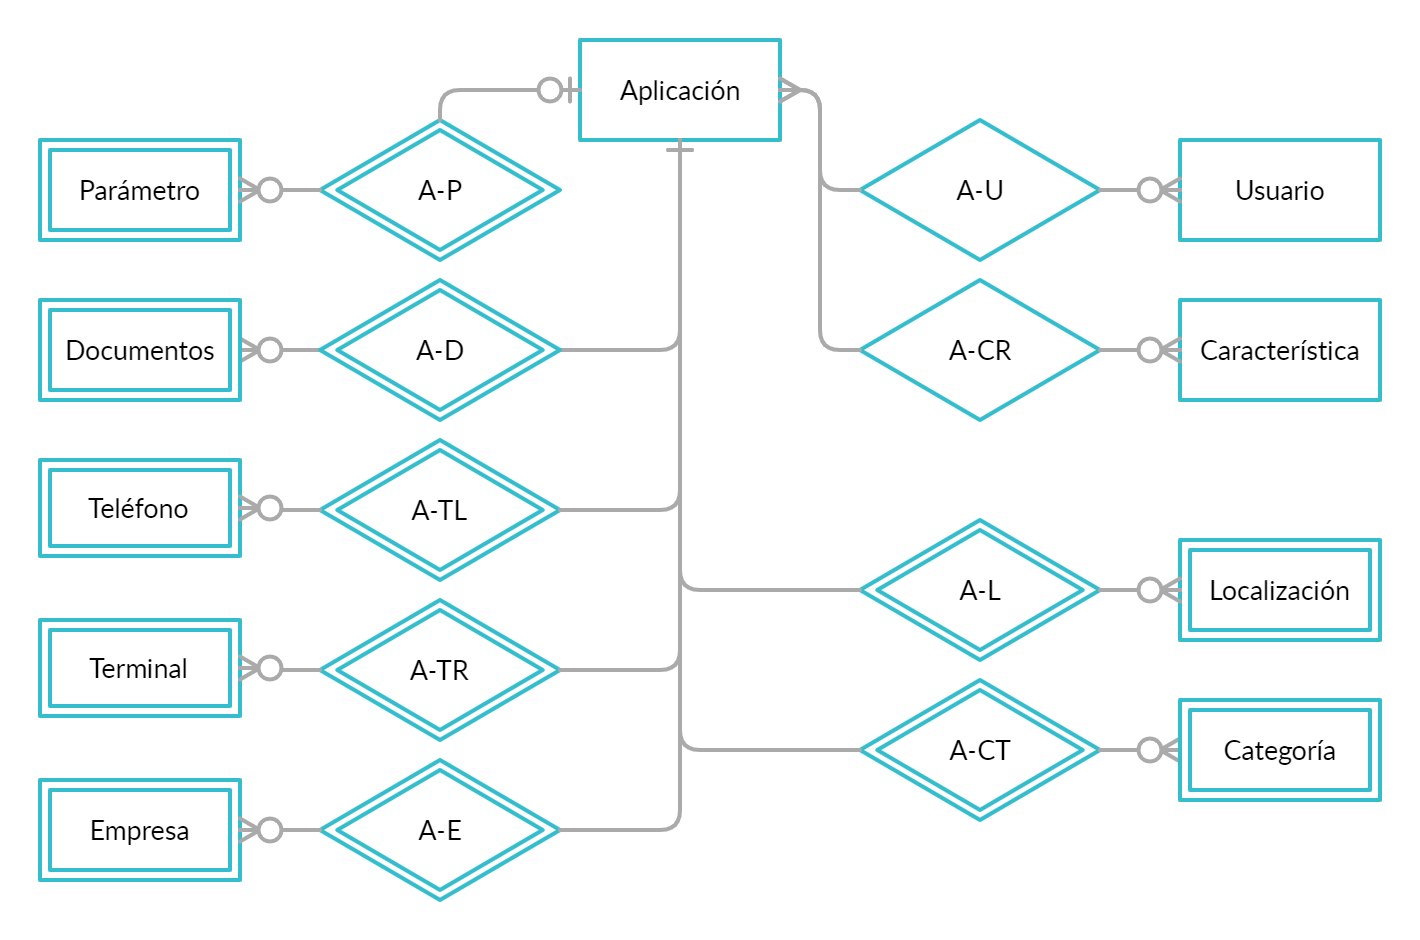
\includegraphics[scale=.31]{PushNews E-R 1}
    \caption{Aplicación como entidad fuerte}
    \label{fig:diagram-entidad-interrelacion-1}
\end{figure}

\begin{figure}[h]
    \centering
    % https://app.creately.com/diagram/FGzbpRaBqk7/edit
    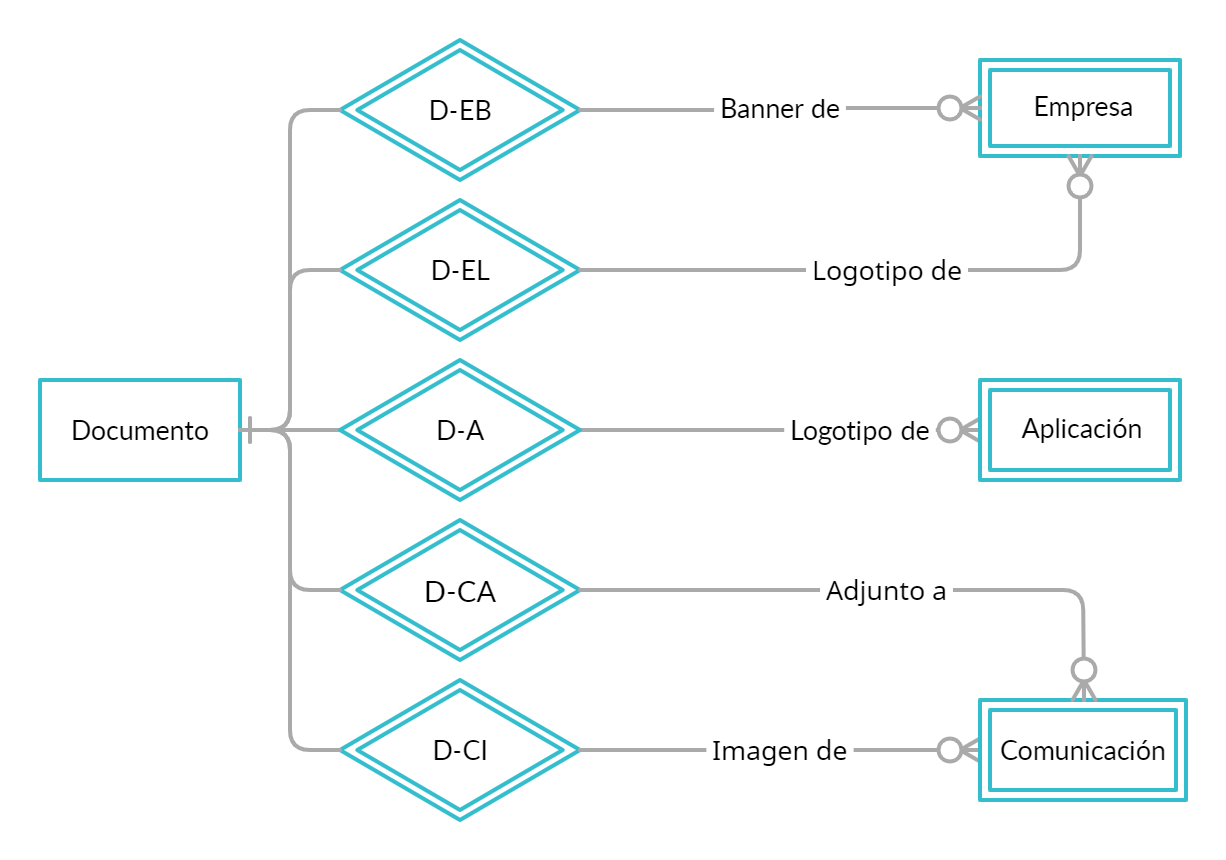
\includegraphics[scale=.31]{PushNews E-R 2}
    \caption{Documento como entidad fuerte}
    \label{fig:diagram-entidad-interrelacion-2}
\end{figure}

\begin{figure}[h]
    \centering
    % https://app.creately.com/diagram/rUhAbYQdpj2/edit
    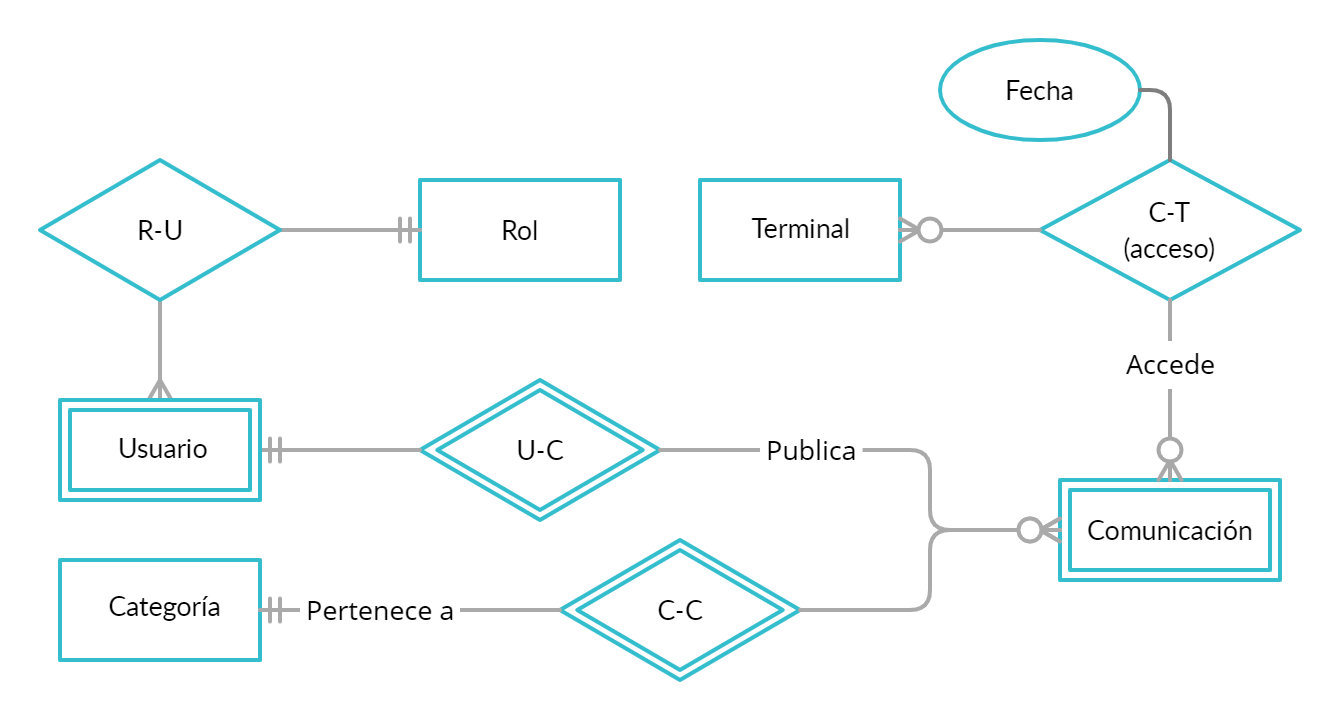
\includegraphics[scale=.31]{PushNews E-R 3}
    \caption{Resto de relaciones}
    \label{fig:diagram-entidad-interrelacion-3}
\end{figure}